\documentclass[conference]{IEEEtran}
\usepackage{amsmath,amssymb,booktabs,graphicx,balance}
\usepackage[hidelinks]{hyperref}
\usepackage{iftex}
\ifXeTeX
\usepackage{fontspec}
\setmainfont{texgyretermes-regular.otf}[BoldFont=texgyretermes-bold.otf,ItalicFont=texgyretermes-italic.otf,BoldItalicFont=texgyretermes-bolditalic.otf]
\setsansfont{texgyreheros-regular.otf}[BoldFont=texgyreheros-bold.otf,ItalicFont=texgyreheros-italic.otf]
\setmonofont{texgyrecursor-regular.otf}[BoldFont=texgyrecursor-bold.otf]
\fi
\hypersetup{pdftitle={Reopening Graph Memory for Coding Agents},pdfauthor={Anonymous working draft}}
\title{Reopening Graph Memory for Coding Agents:\\From Source Events to Missing Addresses}
\author{\IEEEauthorblockN{Anonymous working draft}}
\begin{document}
\maketitle
\begin{abstract}
A coding agent returning to a repository can recover past changes by opening an exact index of their participating files. We demonstrate how the material represented in volatile memory changes the cost of this operation. Visitors inspect an actual shared event, choose between copying bodies and reopening references to a durable journal, then change how a bounded cache describes missing event addresses. All methods return the same ranked files and scores. In a prespecified six-repository holdout with 721 dense queries and a 1\,KiB cache, storing the count and XOR of posting identifiers transferred 20,055 bytes from SQLite, compared with 21,957 for compressed exact postings and 27,411 for ordinary joint LRU. At 4\,KiB exact postings used fewer bytes. The demonstration exposes both outcomes, a compressed-copy counterexample, and the CPU cost of resolving addresses. Its measurements concern the graph store's boundary with SQLite.
\end{abstract}
\section{Introduction}
Consider a coding agent reopening a repository to find tests related to a source file. Its durable memory records an event for each eligible commit and links that event to all Python files changed together. An old change may be useful from several anchor files. Reopening a process discards cached event bodies as well as lists of their addresses. A reader can retrieve these objects again, retain copies in a checkpoint, or carry a small description of how to retrieve them. Each choice can return the same evidence at a different cost.

Change histories have long supported file recommendations~\cite{rose,moonen}. Recent agent-memory demonstrations such as TAPE~\cite{tape} illustrate why searchable temporal structure is useful. Here the database question arises after an agent or developer has already selected a memory query. Which information must cross the process boundary, and which information can a reader reconstruct from objects already present? A near-optimal choice of events inside a copied-body format can leave considerable room for improvement once the representation itself becomes a design variable.

The first console view compares physical encodings for the \emph{same} selected events. It itemizes the bytes written, restored, verified and subsequently fetched, so a visitor can see when copying pays. The second follows an actual query from a source file to commits and a ranked answer. A third assigns a bounded cache to event bodies, posting lists or both. The fourth lets a visitor remove one or two event identifiers and see which missing addresses are identifiable. A six-repository panel tests whether the last representation saves bytes under a fixed budget. All four views run offline from an exported experiment registry.

\section{Durable evidence and the query}
Let an event $e_j$ contain the distinct file identifiers changed in the $j$th eligible commit. We store each body once in an append-only SQLite table keyed by $j$. An inverted list $P_f$ maps file $f$ to its events. The single-anchor query returns the first eight other files under descending score
\begin{equation}
s(f,x)=\sum_{j\in P_f} {\bf 1}[x\in e_j].
\end{equation}
Recent file frequency over 32 source commits and then stable file identifier break ties. Scores may be zero, so a query also sees the prior ordering of all files known at that instant. File identities and event memberships come from earlier commits only. An anchor first appearing in the query commit can therefore be unknown to the reader.

The hot index lets each file retain pointers to its eight newest accepted events. An event body stays accessible to every participant while it has any remaining owner. SQL remains the authoritative fallback when a relevant old event is missing. A file shared with a busy subsystem can consequently benefit from another participant's retention decisions. Releasing the final owner affects both the body table in RAM and all volatile incidence links to that body.

Git history is a proxy for interactions a repository-aware agent could remember. Changed paths need no natural-language labels and permit independent re-execution of every ranked answer. They do not establish that co-change is the best test-selection signal or that showing the results improves generated patches. In a complementary replay on 57 SWE-ContextBench Lite tasks~\cite{swectx}, genuine past read-to-edit associations retrieved the relevant trajectory first in 44 cases, exactly as many as the same addresses without edges. That observation motivates keeping answer quality separate from the cost of restoring an already specified query.

\section{Reopening by reference}
The durable journal contains each immutable body under a stable ID. A snapshot can preserve membership in a selected set without holding the bodies themselves. This is related to separating keys and values in a store~\cite{wisckey}. Here a single value participates in several graph lookups and the decision includes prepaid transmission of a checkpoint to a later process. Our reader binds its packet to the event count and revision, checks its checksum, and rejects obsolete metadata. It assumes the same immutable journal and numbering remain available.

\subsection{Keeping the comparison matched}
We select the eligible set from the hot index at the restart boundary. In one condition, all live events are selected. In the other, we process candidates in decreasing order of a score based on body length, the sum of recent frequencies of its participants, and the bytes of its copy entry. Each candidate must fit the remainder of a 1\,KiB copied-body budget. This budget determines the same set for each recovery method. Every checkpoint uses its natural encoded length, including a 40-byte envelope. Reopening validates a 20-byte source revision.

The methods are a raw body copy, a body copy using the shorter of raw and zlib at level one, an address packet with immediate body loading, and the same packet with loading on first use. The packet chooses the shortest of absolute IDs, gaps, gaps in the complement and a bitmap, including compressed alternatives. In the lazy version each selected body stays pinned after first use until the end of the continuation. Incoming commits use the common eight-event write cache. This pinned policy has a different memory contract from the bounded LRU comparison below.

For a copy of $C$ bytes, a reference packet of $R$ bytes, and $F$ immutable body bytes first required in the continuation, the difference in measured charges is
\begin{equation}
T_{\rm copy}-T_{\rm lazy}=2(C-R)-F .
\end{equation}
The factor of two accounts for writing and loading each packet. The two readers receive the same posting bytes and unselected bodies. Each selected body contributes to $F$ at most once. If their total size is $B$ and there are $k$ bodies, the raw copy contains the absolute IDs, at least one length byte per body, and all $B$ bytes. Absolute IDs are one admissible reference format, so the saving against the raw copy is at least $B+2k$ for a nonempty selection. Compression changes $C$ and can reverse the result.

\begin{table}[t]\centering
\caption{Recovery charges for the same demand-weighted selection. All entries are bytes, including write and load.}\label{tab:restart}
\begin{tabular}{lrrr}\toprule
Method & Original sparse & Holdout sparse & Holdout dense\\
\midrule Raw copy & 82,907 & 11,389 & 41,640\\
Compressed copy & 82,729 & 10,963 & 41,214\\
Eager references & 79,902 & 6,690 & 36,941\\
Lazy references & 79,893 & 5,708 & 36,589\\
\bottomrule\end{tabular}
\end{table}

\subsection{What the visitor can falsify}
The ledger starts with three longer histories and 196 post-restart queries. At that point eagerness costs only nine additional bytes relative to lazy references. The visitor can reset the horizon to zero and see the entire preload charged before the first query. On six previously unused repositories (Table~\ref{tab:restart}), the difference between eager and lazy is larger on the sparse workload. A contrary example is built into the console. Each of 128 events contains 32 common files and one private file. A single request for a common file needs all 4,256 body bytes. The compressed copy costs 1,464 bytes in total, the references 4,484 and the raw copy 9,252. The database returns the same ranked files in all three runs.

A preceding restricted oracle could save at most 33,439 read bytes by selecting copied events at the 1\,KiB operating point on the three longer histories. A causal demand-weighted choice saved 30,078 of those body bytes. That bound constrains which copies to include within a given format. Equation~(2) examines a different choice with the very same events. Once the source journal is available, the earlier ceiling cannot bound the value of all checkpoint representations.

\section{Reconstructing missing addresses}
The next comparison begins from a cold process. A common baseline caches immutable bodies. A stronger ordinary LRU admits both posting lists and bodies under one byte quota. Avoiding a second posting read can be inexpensive, but a large posting may displace many useful bodies. On twelve additional histories and 189 sparse queries, moving from bodies only to joint LRU at 4\,KiB reduced traffic from 14,532 to 11,600 bytes. Both read 6,997 bytes of bodies. At 1\,KiB the same change increased total cost from 16,777 to 17,698 bytes. The visitor can view every project's result at either limit.

\subsection{A small exact certificate}
Suppose the reader has a certified subset $K_f\subseteq P_f$ consisting of the resident bodies that actually include $f$. To find $K_f$, the implementation checks the hot index and scans the bounded resident bodies, charging scan work. For a retained posting summary, store its cardinality $n_f$ and the value $z_f=\bigoplus_{j\in P_f}j$. Confirmed appends update these fields for participating files. Let $d=n_f-|K_f|$. When $d=0$ all IDs are known. When $d=1$ the absent ID equals $z_f\mathbin{\oplus}\bigoplus_{j\in K_f}j$, and an indexed fetch can read its body directly. For $d>1$ the reader requests the authoritative exact list. The guarantee relies on positive set membership, distinct event IDs, consistent updates and a common immutable snapshot. Without the subset condition, one missing and one spurious ID can cancel the cardinality difference.

\begin{figure}[t]\centering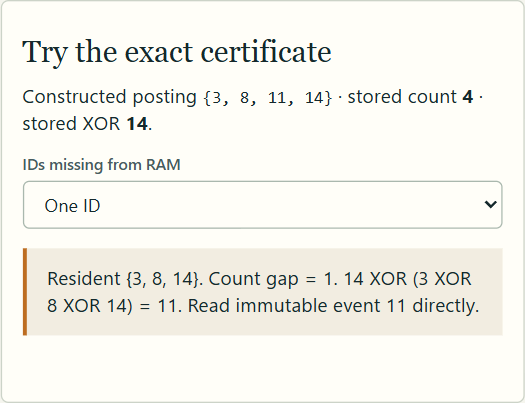
\includegraphics[width=.88\columnwidth]{certificate.png}
\caption{The offline console lets a visitor remove zero, one or two IDs from an explicitly constructed posting. At two missing IDs the source list must resolve the ambiguity.}\label{fig:ui}
\end{figure}

Count-and-XOR cancellation is classical in set reconciliation, including invertible lookup tables~\cite{iblt}. Our experiment tests the allocation it enables in a coding-history query. The exact baseline also gets compact postings and can use body space freed by compression. We keep ordering, capacity accounting and source data fixed. A count-only control isolates coverage tests at $d=0$. A control based on two power sums can reconstruct up to two missing IDs at a higher metadata and arithmetic cost. No extra reverse index is provided without a budget charge. The test asks whether sacrificing full postings to preserve bodies pays under these constraints.

\subsection{Frozen transfer to six new repositories}
We fixed the primary contrast, model-free query rule and six public projects before computing holdout outcomes. Up to 1,024 first-parent transitions are used for isort, Rich, inflect, marshmallow, numpydoc and Pendulum. A source commit with 2--64 Python paths generates an eligible event. The dense rule generates queries from eligible commits after the first 64 source transitions. The sparse rule samples by commit hash in the second half of the source stream. Queries use a reproducible hash-selected anchor and run before the corresponding event is appended. Restart occurs halfway through eligible events. The two workloads can overlap and share repository history.

\begin{table}[t]\centering
\caption{SQLite payload after reopening on six held-out repositories. Capacities apply to additional packed LRU state.}\label{tab:xor}
\begin{tabular}{lrrrr}\toprule
Workload & Budget & Joint & Exact & Count + XOR\\\midrule
Dense, 721 & 1 KiB & 27,411 & 21,957 & 20,055\\
Dense, 721 & 4 KiB & 5,911 & 5,911 & 7,725\\
Sparse, 60 & 1 KiB & 4,006 & 3,746 & 4,048\\
Sparse, 60 & 4 KiB & 3,520 & 3,520 & 3,951\\\bottomrule
\end{tabular}
\end{table}

In the primary setting the certificate saved 1,902 bytes or 8.66\% against compressed exact postings. Body traffic fell by 2,816 bytes while posting traffic rose by 914 bytes. A count-and-XOR query identified exactly one missing ID 51 times. Its main aggregate benefit came from a different balance of retained bodies and lists, so a count of certificate successes alone is insufficient to explain the saving. Three repositories improved, two tied and one worsened (Fig.~\ref{fig:hold}). At 4\,KiB both methods read the same 3,217 body bytes, and exact lists saved posting traffic. On the sparse holdout only one query recovered a single ID. Table~\ref{tab:xor} displays those regimes alongside the primary result.

\begin{figure}[t]\centering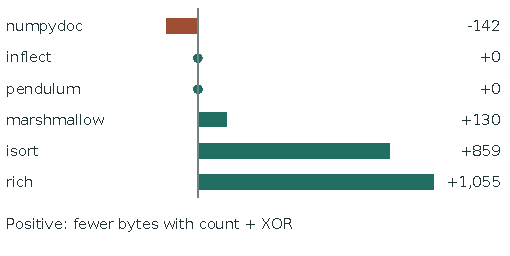
\includegraphics[width=\columnwidth]{holdout.pdf}
\caption{Paired dense holdout results for 1\,KiB. Each bar gives compressed-exact bytes minus count-and-XOR bytes for one repository.}\label{fig:hold}
\end{figure}

\subsection{Transport and CPU costs}
A second control allows the full posting representation to append efficiently and makes membership testing cheaper for the certificate. On the same dense holdout at 1\,KiB, measured payload changed from 22,186 to 20,063 bytes. Reading and maintaining the state took 56.32 versus 57.87\,ms. This limits the performance claim: a reduction in logical bytes can coexist with a longer execution. On one loopback implementation of the original underlying readers, bidirectional traffic changed from 36,582 to 33,180 bytes and calls from 688 to 670. With no injected delay, reads took 176.62 and 188.77\,ms respectively. At 2\,ms imposed per call, they took 1,849.81 and 1,829.36\,ms. The result depends on local encoding, batching and round-trip latency. Technical timing blocks quantify system variability without creating additional independent repositories.

\section{Demonstration and reproducibility}
The browser application works without network access. In \emph{Restart ledger}, a visitor selects a cohort, repository, horizon and event-selection budget, then reads the components of each charge. \emph{Event inspector} opens a measured request. The first step reveals the selected historical bodies fetched for the first time, including commit prefixes, participant counts and encoded lengths. The second step reveals the top eight file paths with scores. Previously pinned bodies and new journal events can also supply evidence. This inspection connects the database's transfer counts to a recognizable repository action.

In \emph{Cache budgets}, changing the quota exposes the sign reversal between caching only bodies and caching both postings and bodies. In \emph{Missing event IDs}, the visitor controls a small posting with IDs $\{3,8,11,14\}$ and compares exact recovery against the holdout registry (Fig.~\ref{fig:ui}). Removing 11 leaves a single solution. Removing 8 and 11 leaves a residual XOR of 3. The alternatives $\{8,11\}$ and $\{4,7\}$ then have the same cardinality and XOR, forcing a fallback. The measured panel uses real traces and can switch repositories independently of the constructed explanation.

The downloadable artifact contains committed protocols, pinned history data, per-query SQLite work, standalone UI generation and independent checks. For the original nine repositories and the two workloads on twelve additional repositories, a separate implementation regenerated the exact ranking of 2,940 queries from raw Git events. Another audit intercepted returned SQLite BLOBs in 64 fresh runs covering 5,664 answers, including empty and alternate subsets. A changed revision, corrupt checksum or different source length forced exact fallback in close--reopen checks. The corpus characterizes exact storage retrieval under one writer. Physical page I/O and end-to-end coding-task success require separate measurements.

\balance
\subsection{Reading the causal comparison}
The ledger and the bounded-cache panel answer different intervention questions. First we keep the selected event IDs fixed while varying their representation. This holds the logical evidence constant and exposes how much of the gain comes from encoding. In the cache panel, changing the size of a posting can affect which bodies survive subsequent admissions. Matching the total byte capacity is then more informative than matching the number of retained objects. Reserving the same number of postings for both treatments would suppress the very mechanism under test. The common source and exact-answer checks keep query semantics fixed as residency diverges.

A project-level view prevents a large repository from becoming the entire result. In the dense 1\,KiB holdout, Rich accounts for 1,055 of the 1,902 net bytes saved; isort contributes 859. Marshmallow contributes 130, while numpydoc uses 142 additional bytes and the remaining two repositories tie. These are six units of transfer evidence. Repeated requests within Rich can share hot objects and should not be counted as independent evidence for generalization to new repositories. The aggregate is relevant to servicing the actual workload, whereas the paired breakdown describes its heterogeneity. A visitor can reproduce each delta by switching the repository selector in the last tab.

The format and the query schedule also matter independently. When a process never receives a second query, carrying an unnecessary posting consumes space that might have held a useful body. When many upcoming queries share the same file, retaining the exact list can amortize its larger size. In the 4\,KiB dense result, the two readers return exactly the same body payload, so all 1,814 additional XOR bytes come from fetching postings. At 1\,KiB the body advantage was sufficient to pay the extra posting charge. The direction change is visible without attributing a universal value to a checkpoint byte or to one recovered address.

\subsection{Limits of replay}
The journal source uses commit history and an append-only, single-writer view. It does not simulate every action that an autonomous coding agent makes. The cutoff at 64 paths and the fixed hashing rule determine which questions are present. A different objective, such as finding the best integration test per prompt token, would also require evaluating retrieval relevance and downstream testing behavior. Membership certification cannot repair missing or incorrectly extracted evidence from an upstream memory writer.

A separate exercise on 108 recorded SWE-agent sessions illustrates this distinction for actual editor reads. We restarted after half the observed editor windows and transferred previously verified equalities between line addresses. The new process could read one member of an equality class on demand and reuse its contents for another member, while invalidating all equalities at mutation barriers. Across 436 post-restart windows, that policy eliminated 239 source-line reads. However, the resulting 2,429-byte decrease in compressed replies did not cover 10,348 bytes paid for writing and reopening the equality metadata. This is a trace-replay diagnostic with no trusted filesystem generation for an external change during downtime. It supports a narrower conclusion about the cost boundary: eliminating an operation does not by itself pay for a memory representation.

\section{Conclusion}
For a persistent graph of shared Git changes, the unit of recovery matters. Stable references have a provable logical-byte advantage over the chosen raw-copy format. A compressed copy can still win, and allocating a bounded cache to endpoint summaries helps only in particular workloads. The demonstration lets a visitor verify the address recovery, inspect the original events and identify the regime where the strong exact baseline is preferable.

\section*{Acknowledgment}
OpenAI Codex assisted with implementation, analysis and drafting. This anonymous research draft has not been submitted.

\begin{thebibliography}{6}
\bibitem{rose} T. Zimmermann, P. Weisgerber, S. Diehl, and A. Zeller, “Mining version histories to guide software changes,” in \emph{ICSE}, 2004, pp. 563--572. \href{https://doi.org/10.1109/ICSE.2004.1317478}{doi:10.1109/ICSE.2004.1317478}.
\bibitem{moonen} L. Moonen, S. Di Alesio, D. Binkley, and T. Rolfsnes, “Practical guidelines for change recommendation using association rule mining,” in \emph{ASE}, 2016, pp. 732--743. \href{https://doi.org/10.1145/2970276.2970327}{doi:10.1145/2970276.2970327}.
\bibitem{tape} C. Luo, Q. Liu, W. Zhang, and Y. Gao, “TAPE: A temporal graph-based memory system for personal LLM agents,” in \emph{ICDE}, 2026, pp. 4168--4171. \href{https://doi.org/10.1109/ICDE65706.2026.00318}{doi:10.1109/ICDE65706.2026.00318}.
\bibitem{wisckey} L. Lu, T. S. Pillai, A. C. Arpaci-Dusseau, and R. H. Arpaci-Dusseau, “WiscKey: Separating keys from values in SSD-conscious storage,” in \emph{FAST}, 2016, pp. 133--148.
\bibitem{iblt} M. T. Goodrich and M. Mitzenmacher, “Invertible Bloom lookup tables,” \emph{arXiv:1101.2245}, 2011, revised 2015. \href{https://arxiv.org/abs/1101.2245}{arXiv}.
\bibitem{swectx} J. Zhu et al., “SWE Context Bench: A benchmark for context learning in coding,” \emph{arXiv:2602.08316}, 2026. \href{https://arxiv.org/abs/2602.08316}{arXiv}.
\end{thebibliography}
\end{document}
